\documentclass{standalone}
\usepackage{tikz}
\usepackage{amsmath}
\usepackage{xcolor}
\usetikzlibrary{arrows.meta, decorations.pathreplacing, backgrounds, positioning, calc}
% Define custom colors
\definecolor{softyellow}{HTML}{F2D648}
\definecolor{dustyblue}{HTML}{9EB9D4}
% Define styles for common elements
\tikzset{
  energy level/.style={very thick, blue!80!black},
  atom X/.style={circle, fill=softyellow, draw=black, minimum size=0.5cm, line width=1.5pt},
  atom M/.style={circle, fill=dustyblue, draw=black, minimum size=0.6cm, text=black, line width=1.5pt},
  bond/.style={thick, gray!60},
  dashed bond/.style={dashed, gray!60}
}
\begin{document}
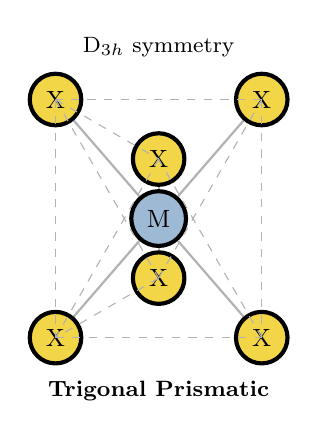
\begin{tikzpicture}[scale=1.4, >=Stealth, font=\small]
  % --- Energy axis and other elements would go here ---
  
  % --- Trigonal prismatic geometry with complete dashed lines ---
  \begin{scope}[xshift=6.2cm, yshift=2cm, scale=1.2]
    % Central transition metal atom (Mo)
    \node[atom M] (M) at (0,0) {M};
    
    % Define chalcogen positions (S atoms)
    \def\Rinner{0.9}  % Distance from center to ligands
    \def\Zshift{0.45} % Vertical shift for top/bottom triangles
    
    % Top triangle of chalcogen atoms (S)
    \foreach \angle/\idx in {30/1, 150/2, 270/3} {
      \coordinate (X-top-\idx) at ({\Rinner*cos(\angle)}, {\Rinner*sin(\angle)+\Zshift});
      \draw[bond] (M) -- (X-top-\idx);
      \node[atom X] at (X-top-\idx) {X};
    }
    
    % Bottom triangle of chalcogen atoms (S) - staggered arrangement
    \foreach \angle/\idx in {90/1, 210/2, 330/3} {
      \coordinate (X-bottom-\idx) at ({\Rinner*cos(\angle)}, {\Rinner*sin(\angle)-\Zshift});
      \draw[bond] (M) -- (X-bottom-\idx);
      \node[atom X] at (X-bottom-\idx) {X};
    }
    
    % Vertical connections to show prism structure - ALL THREE SIDES
    \draw[dashed bond] (X-top-1) -- (X-bottom-3);
    \draw[dashed bond] (X-top-2) -- (X-bottom-1);
    \draw[dashed bond] (X-top-3) -- (X-bottom-2);
    
    % Triangular faces - top triangle
    \draw[dashed bond] (X-top-1) -- (X-top-2);
    \draw[dashed bond] (X-top-2) -- (X-top-3);
    \draw[dashed bond] (X-top-3) -- (X-top-1);
    \draw[dashed bond] (X-top-2) -- (X-bottom-2);
    
    % Triangular faces - bottom triangle
    \draw[dashed bond] (X-bottom-1) -- (X-bottom-2);
    \draw[dashed bond] (X-bottom-2) -- (X-bottom-3);
    \draw[dashed bond] (X-bottom-3) -- (X-bottom-1);
    
    % Labels
    \node[font=\footnotesize\bfseries] at (0,-1.3) {Trigonal Prismatic};    
    % Optional: Add symmetry label
    \node[font=\footnotesize, black] at (0,1.3) {D$_{3h}$ symmetry};
  \end{scope}
  
  % --- Rest of the diagram would go here ---
\end{tikzpicture}
\end{document}
